\chapter{Introduction and Motivations}\label{ch:introduction}


\begin{flushright}
		\emph{The series is divergent, therefore we may be able \\ to do something with it.}\\
			- Oliver Heaviside
\end{flushright}

\vspace{0.6cm}


Medical image registration is a set of tools and techniques oriented to solve the problem of determining correspondences between two or more images acquired from patients scans. Its development is a creative field that has seen the application of a growing number of mathematical theories in the research of customizations and improvements of precision and computational time. It has a wide range of applications: for example it can be used in lungs motion correction \cite{mcclelland,mcclelland2011inter}, in Alzheimer disease diagnoses \cite{prados2015measuring, fox1997brain, gauthier2012prevention}, and image mosaicing \cite{vercauteren2006robust, szeliski1994image}.  

Determining correspondences between images is often presented as an ill-posed problem: transformations between anatomies are not unique, and the impossibility to recover spatial or temporal evolution of an anatomical transformations, starting only from few images over a long time makes any validation a difficult, if not an impossible task. 

The most important feature in image registration algorithms is the \emph{deformation model}: the set of transformations chosen to model the anatomical deformations. This is aimed constrain deformations according to the task that the registration algorithm has to perform and to adapt to the nature of the objects represented by the images (see \cite{ibanez2003itk} for a presentation of the image registration framework and \cite{Sotiras:survey:13} for a recent survey in medical image registration). 

% % % % % % % % % % % % % % % % % % % % % % % % % % % % % % % % % % % % % %
% % % % % % % % % % % % % % % % % % % % % % % % % % % % % % % % % % % % % %
\section{Choosing the Deformations: Diffeomorphisms}

If the registration algorithm is meant to model physical transformations that preserve distances, orientations and angles, then the deformation model can be bounded to the group of rigid body transformations \cite{gallier2011geometric}. The consequent registration algorithm, called \emph{rigid-registration algorithm}, will be suitable for example to compensate the motion in a rapid sequence of scans, or to investigate small differences that occurs in longitudinal studies.

If the algorithm is meant to model transformations that only preserves topology, then the transformations must allow more freedom than the one chosen for the rigid case. It is in this context that arises the mathematical object of \emph{diffeomorphism} over $\Omega\subseteq \mathbb{R}^{d}$. This is defined as a bijective differentiable map from $\Omega$ to itself, with differentiable inverse, and is particularly well suited to model non-rigid deformation between images. Algorithms involving diffeomorphisms are called \emph{diffeomorphic registration algorithms}.

In both cases, the transformation belongs to a \emph{group structure} (see \cite{artin2011algebra}). Here the only operation of composition is defined, and for mathematical reasons it is not possible to define any norm or mean. A strategy to solve this problem is to consider the group with a differentiable manifold structure compatible with the operation of composition, called \emph{Lie group}, and to consider the linear approximation of its element in the tangent space, called \emph{Lie algebra}. In this vector space it possible to define a norm and therefore to compute statistics. This Matster Thesis is strongly based on the mathematical concepts just introduced, but a short formal introduction of each of them would require to overcome at least twice the available number of worlds. The interested reader can refer to the wide literature, starting for example from \cite{lee2012introduction, arnold2006ordinary, warner, do1976differential}.

Considering the group of diffeomorphisms as a Lie group was proposed in medical imaging for the first time in $2006$, with the name of \emph{log-Euclidean framework} \cite{Arsigny:MRM:06}. The passage from the structure of the Lie group to the structure of the Lie algebra is performed using two numerical algorithm for the computation of the \emph{Lie exponential} (the map from the Lie group to the Lie algebra) and the \emph{Lie logarithm} (the map from the Lie algebra to the Lie group).

It is important to notice that after a transformation has moved from the Lie group to the Lie algebra, it is not possible anymore to compute the composition with another element of the group unless it is not exponentiated again. The composition can be performed only in the Lie group, and there is no operation available in the Lie algebra that reflects the feature of the composition of the corresponding transformations.

It is in this context that arises the abstract concept of log-composition, whose numerical computations are the main aim of this research.


% % % % % % % % % % % % % % % % % % % % % % % % % % % % % % % % % % % % % %
% % % % % % % % % % % % % % % % % % % % % % % % % % % % % % % % % % % % % %
\section{Introducing the Log-composition and the BCH formula}

% 
Indicating with $\exp$ the Lie exponential  and with $\log$ the Lie logarithm, the log-composition is defined for each couple of vectors $\mathbf{v}_1$, $\mathbf{v}_2$ belonging to the domain of $\exp$ as
\begin{align}\label{eq:bch_problem}
\mathbf{v}_1 \oplus \mathbf{v}_2 := \log(\exp(\mathbf{v}_1)\circ\exp(\mathbf{v}_2))
\end{align}

\begin{figure}[!ht]
	\centering
	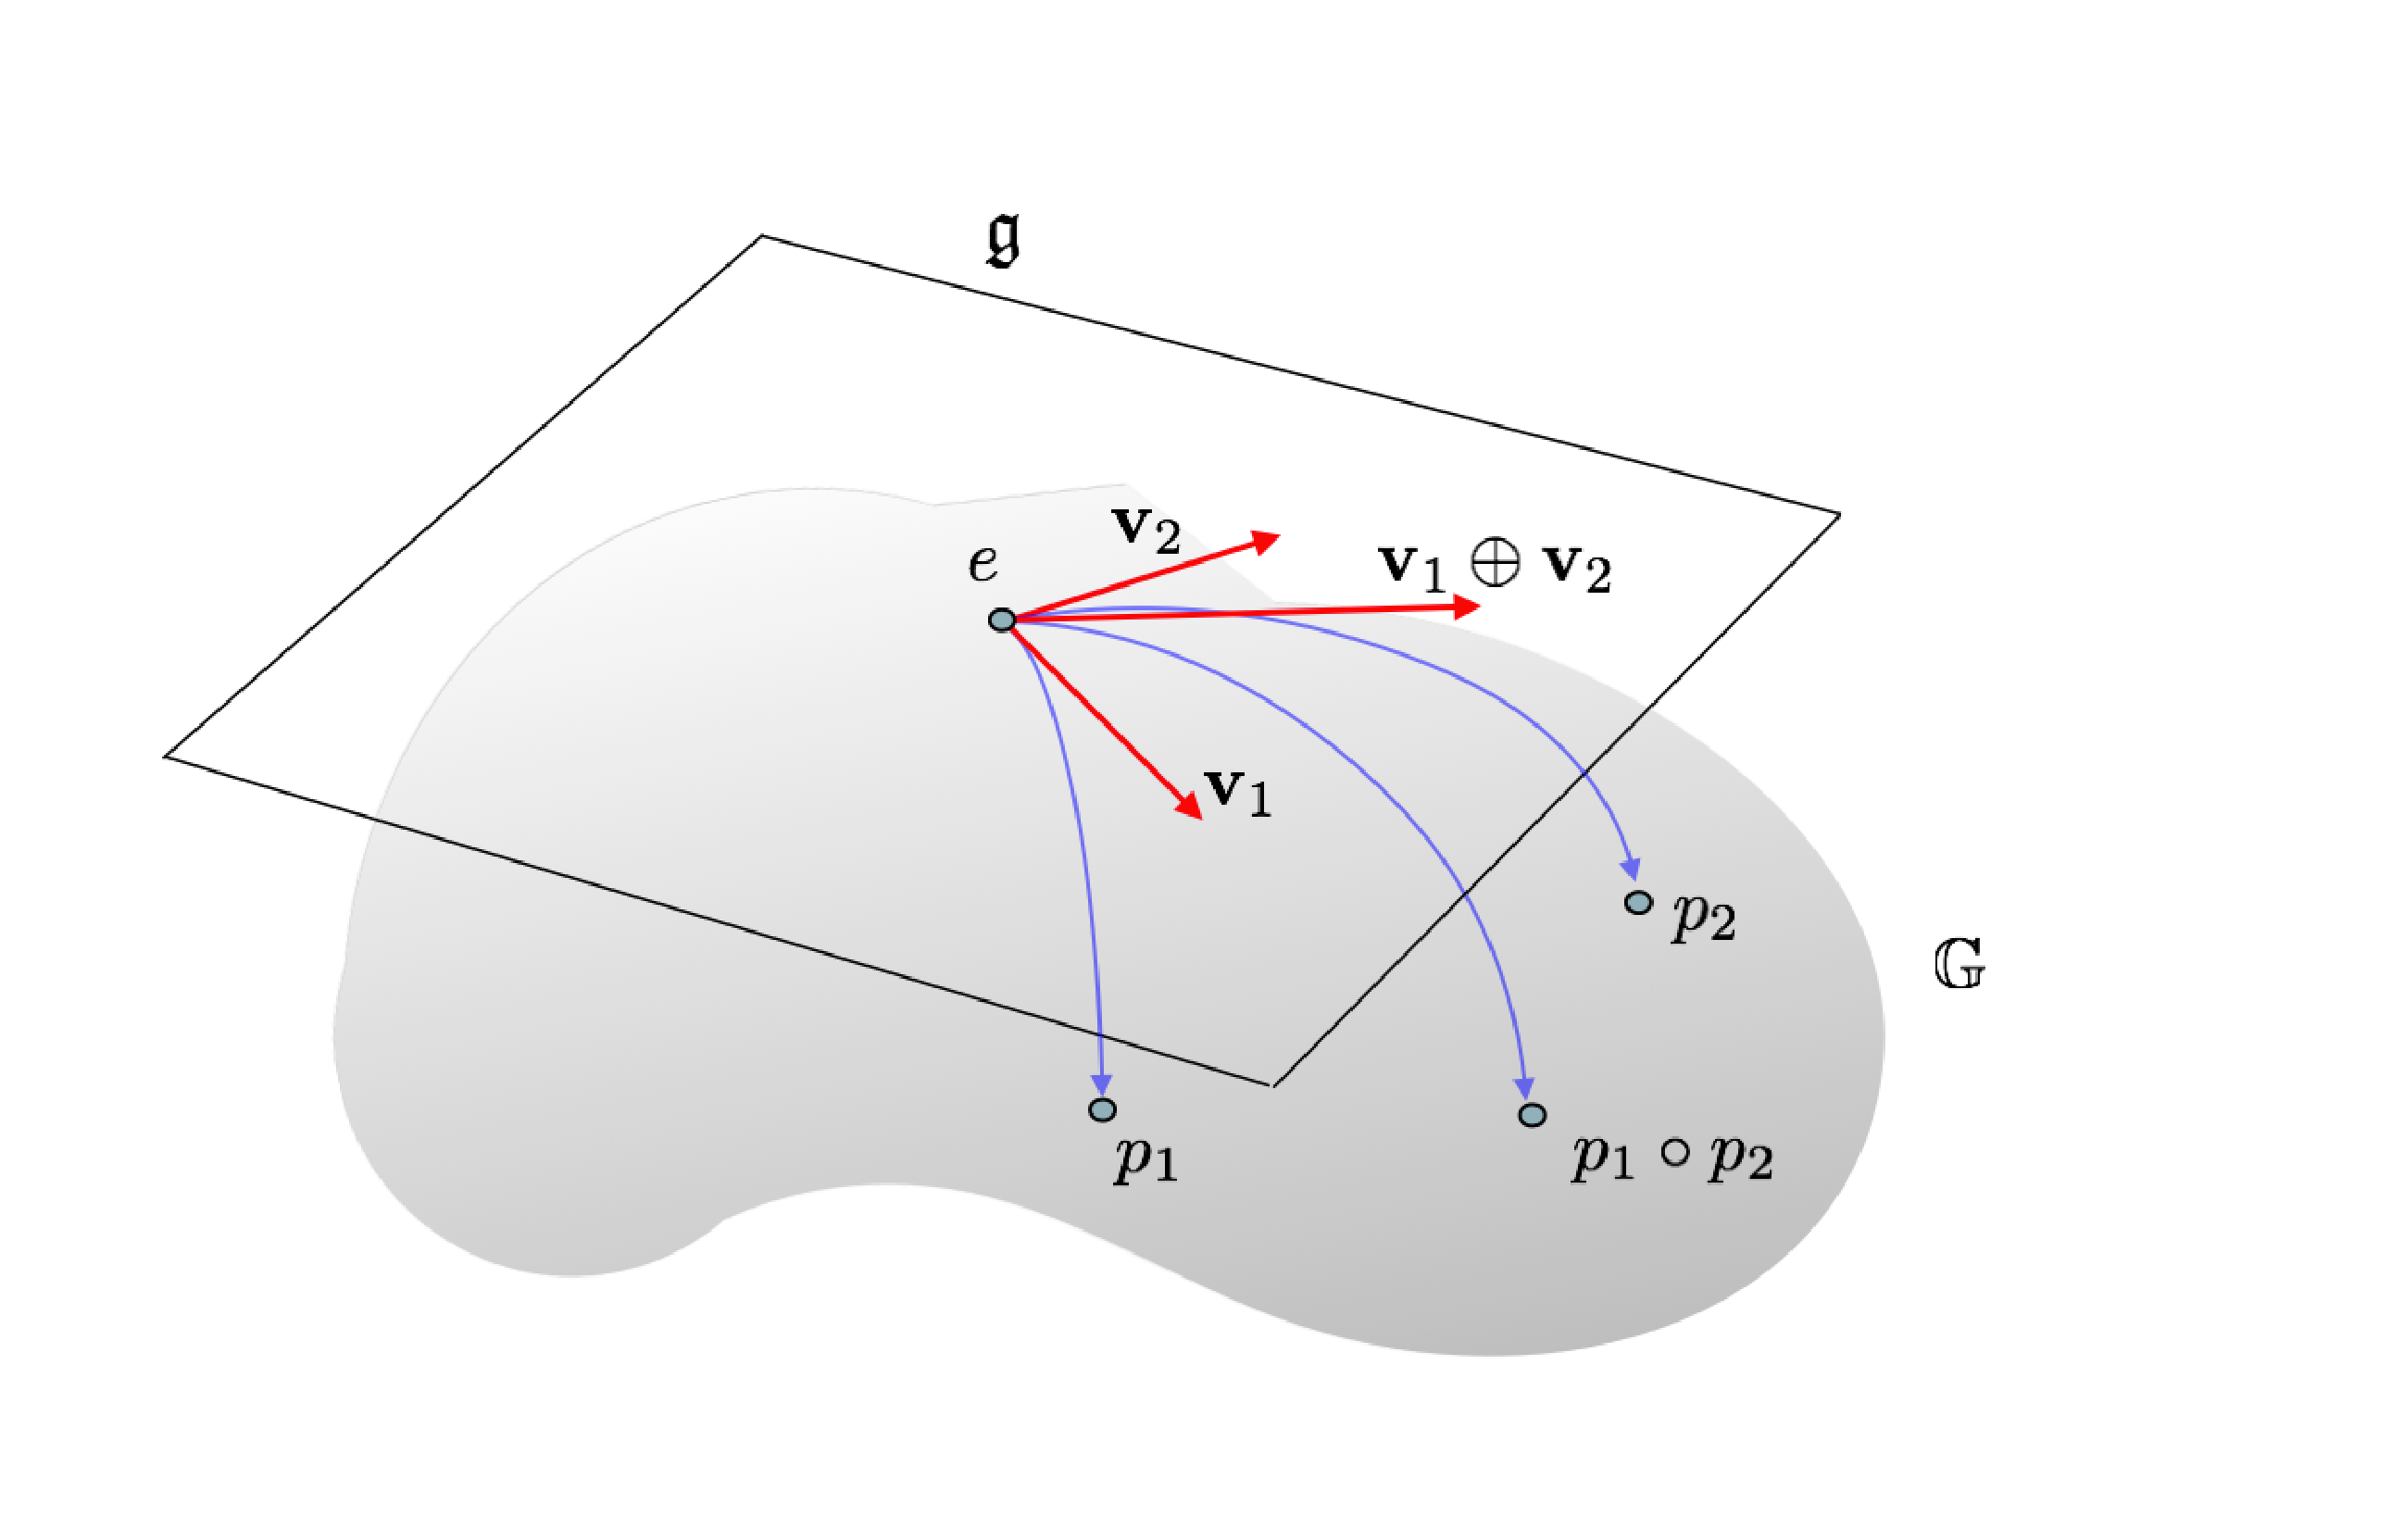
\includegraphics[scale=0.35]{figures/log_composition.pdf}
	\caption{graphical visualization of the Lie log-composition $\mathbf{v}_{1}\oplus \mathbf{v}_{2}$. The gray surface represents a Lie group and its tangent plane represents its Lie algebra. }
	\label{fig:composition}
\end{figure}

% schematical overview
A schematic perspective of the formula can be visualized in figure \ref{fig:composition}. The Lie group, indicated with $\mathbb{G}$, is represented by the gray surface, while the Lie algebra, indicated with $\mathfrak{g}$, is represented by the tangent plane at the identity $e$.
Starting from the two vectors $\mathbf{v}_1$ and $\mathbf{v}_2$ in $\mathfrak{g}$, their log-composition provides the vector that corresponds to the composition of the corresponding transformation of the initial vectors. 

% 
The analytic solution to the log-composition is provided by the BCH formula, when both the Lie exponential and Lie logarithm can be expressed in power series:
\begin{align*}
BCH(\mathbf{u},\mathbf{v}) 
= 
\mathbf{u} + \mathbf{v} + \frac{1}{2}[\mathbf{u},\mathbf{v}] + \frac{1}{12}([\mathbf{u},[\mathbf{u},\mathbf{v}]]
+ [\mathbf{v},[\mathbf{v},\mathbf{u}]]) - \frac{1}{24}[\mathbf{v},[\mathbf{u},[\mathbf{u},\mathbf{v}]]] +... 
\end{align*}
Each of its term is defined by an infinite series of growing nested Lie bracket.

%
There are many issues, both theoretical and practical that prevent from the direct use of this formula. The fist and most obvious is that it is an infinite series whose truncations does not possess any asymptotic behaviour.
In addition, even considering a large enough number of term, the Lie bracket of two tangent vector of the Lie group of diffeomorphisms involves the computation of the Jacobian matrices: these are not straightforward and raises some issues presented in section \ref{se:jacobian_problem}.

On the theoretical side, the proof of the BCH is based on the fact that Lie logarithm and exponential have to be expressed in power series. This happen only when the Lie group and its Lie algebra are subsets of a bigger algebra that contains them both. In the case of matrix Lie group (see \cite{hall2015lie} for its definition) this always happen, but in the case of diffeomorphisms, this happens only thanks to some theoretical arrangements presented in section \ref{se:svf}.
 
Aim of this research is to present some numerical methods for the computation of the log-composition that avoid the use of the truncated BCH. One of these methods, here presented for the first time, is based on a geometrical construction on the differentiable manifold of the transformation that utilizes the parallel transport (see section \ref{se:pt}).

Results are not only examined on the Lie group of diffeomorphisms, but also on the matrix Lie group of rigid body transformation of the plane. In this second structure is possible to evaluate the performance on a space where all the closed form are known and the ground truth are known.

% % % % % % % % % % % % % % % % % % % % % % % % % % % % % % % % % % % % % %
% % 
% % % % % % % % % % % % % % % % % % % % % % % % % % % % % % % % % % % % % %
\section{Feasible Applications of the Log-composition in Medical Imaging}
% Quali sono le applicazioni pratiche della log composition
One of the reasons why mathematics is considered a powerful tool is consequence of the fact that a concept defined to solve a problem can, at the same time, be used to solve other problem of different origin and nature - the \emph{unreasonable effectiveness of mathematics in the natural sciences}, also known as Wigner principle \cite{wigner1960unreasonable}. This makes every tool developed in the domain of abstraction a versatile tool, but at the same time difficult to understand.

The log-composition has been defined in this chapter from the problem of the computation of the statistics on the group of diffeomorphisms, but its use is not limited to perform only this task.

In medical imaging there are several other situations in which fast and accurate computation of the log-composition can be used:
\begin{enumerate}
	\item Diffeomorphic demons \cite{vercauteren2007non} and log-demons algorithm \cite{vercauteren08}. In particular in the log-demons, the update at each of the iterative step is computed in the tangent space, using an equivalent formulation of the log-composition. 
	\item Fast computation of the logarithm computation \cite{Bossa:08}. Details of this algorithm are a part of this research and are discussed in chapter \ref{ch:log_algorithm}.
	\item Calculus on diffusion tensor \cite{Arsigny:MRM:06}. The logarithmic multiplication $\odot$ and the logarithmic scalar multiplication $\otimes$ provides the Lie group with a structure of vector field. The log-composition $\oplus$ here proposed provides the Lie algebra with a structure that reflects the composition of the group.  
	\item Image set classification \cite{huanglog}. As based on the log-euclidean framework, could exploit the property of having the group composition in the tangent space.
	\item Computation of the the discrete ladder for the parallel transport \cite{Lorenzi:discrete_ladders:14}. An equivalent of the log-composition is utilized for the computation of the parallel transport. Reversing the procedure, the parallel transport can be utilized for the computation of the log-composition.
\end{enumerate}	

Before moving to the next chapter, aimed to present the numerical techniques for its computation, it is important to spend a couple of words about the infinite dimensional Lie groups.

% % % % % % % % % % % % % % % % % % % % % % % % % % % % % % % % % % % % % %
% % 
% % % % % % % % % % % % % % % % % % % % % % % % % % % % % % % % % % % % % %
\section{A Short Remark about the Lie Group of Diffeomorphisms}

So far we have talked about the group of diffeomorphisms as a Lie group in a natural way, without underline any particular feature of this concept. Actually, the topic of infinite dimensional Lie gorup is an open field of research whose development has not yet reach a definitive formalization.
Aimed to presenting the theoretical problem and difficutlies as well as how we deal with them in this Master Thesis, we retrace the main historical steps and some of the most significant important approaches.

The first attempt to provide some handles to the group of diffeomorphisms for easy manipulation was done for the first time in 1966 by Vladimir Arnold \cite{arnold1966geometrie} (consider also the equivalent \cite{arnold1998topological}, more readable for non-French speakers). To solve differential equation in hydrodynamic, the set of diffeomorphisms $\text{\emph{Diff}}$ is considered as a Lie group possessing a Lie algebra. This assumption is not formally followed in accordance to the problem-oriented nature of this paper. 

Subsequent steps in the exploration of the set of diffeomorphisms as a Lie group, and in the attempt of finding a formalization can be found in \cite{marsden1970hamiltonian, ebin1970groups, omori1970group, michor1980manifolds, leslie1983lie}. A state of the art of  infinite dimensional Lie group in the early eighties can be found in \cite{Milnor:84:remarks}, while more recent results and applications on diffeomorphisms has been published in \cite{ovsienko1992integrals, bauer2010sobolev, schmid2010infinite,  bauer2011geodesic}.

Considering an infinite dimensional group as a differentiable manifold implies the idea of having each of its elements in local correspondence with some generalized \lq\lq infinite-dimensional Euclidean\rq\rq\phantom{z}space. Attempts to set this correspondence showed that, the transition maps are smooth over the Banach spaces. This led to the idea of Banach Manifolds. It has been shown \cite{khesin2008geometry} that the group of diffeomorphisms defined as a manifold does not belongs to the category of Banach manifold but requires an even more general space on which the transition maps are smooth: the Frechet space. Here, important theorems from analysis, as the inverse function theorem, the Frobenius theorem, or the main results from the Lie group theory in a finite dimensional settings, as Lie correspondence theorems, do not hold anymore. 

These difficulties led some researchers in approaching the set of diffeomorphisms from other perspectives: 
for example, instead of treating $\text{\emph{Diff}}$ as a group equipped with differential structures, it is seen as a quotient of other well behaved groups \cite{wojtynski1994one}. In other cases, as in \cite{marsden1970hamiltonian} first and in \cite{milnor1984remarks} later, Banach spaces are substituted with more general locally convex spaces to underpin the definition of smooth manifolds (an formal introduction to the infinite dimensional linear Lie groups, group of smooth maps and group of diffeomorphisms can be found in \cite{neeb2006infinite}).

For the medical imaging purposes, it is not necessary to consider the general theory of infinite dimensional manifolds. Keeping the initial Arnold's problem-oriented perspective, the interest are only about the diffeomorphisms defined on a compact subset $\Omega$ of $\mathbb{R}^d$. Without denying the importance of fundamentals and underestimating the doors research for generalized infinite dimensional Lie group may open, on the formal side we will approach the matter in as similar way of what has been done in set theory: we will use a \emph{naive approach} to infinite dimensional Lie group. Here the fundamental definition of infinite dimensional Lie group is a generalization of the finite dimensional case of matrices, and it is left more to the intuition than to a robust formalization. 









